Information systems (IS) have always tried to model parts of reality. To achieve this modelling, IS contain data representing properties of real-world objects or concepts~\cite{JoseEnriquePons2012},~\cite{Billiet2012}. As time is an essential aspect of many real-world objects or concepts, IS often contain data representing temporal notions which describe such temporal properties~\cite{Bolour1982},~\cite{VanderCruyssen1997}. Such temporal notions usually take the form of either instants~\cite{Jensen1998}, which can informally be seen as infinitely short `moments' or `points' in time, or time intervals~\cite{Jensen1998}.

Data are often produced by humans, but human-made data are prone to imperfections: some data may be vague, imprecise, incomplete, contradictory or uncertain. Data representing temporal notions may contain such imprecisions too~\cite{Devos1994},~\cite{Dubois2003},~\cite{JoseEnriquePons2012},~\cite{Billiet2012}. The work presented in this paper is specifically concerned with time intervals (and as a special case: instants) subject to uncertainty.

Generally, one of the most important purposes of an IS is to allow the retrieval of information or knowledge deduced from its data. Such retrieval is usually done by querying the IS and examining or analyzing the query results or by visualizing the contents of the IS, querying this visualization and examining or analyzing the resulting visualization(s).

Of course, when temporal information is represented in an IS, querying this IS may have a temporal aspect too. Usually, querying such an IS is conceptually done by specifying one or more time indications and requesting information that is in a specific relationship with these indications, where the semantics of these relationships are specifically temporal~\cite{Billiet2012},~\cite{JoseEnriquePons2012},~\cite{Pons2012a}. Thus, some existing proposals have considered groups of basic relationships between time indications used to construct and express specific temporal relationships~\cite{Medina1994},~\cite{Schockaert2008}. Notably, Allen~\cite{Allen1983} presented a reasoning framework containing all semantically usefull basic temporal relationships between time intervals (and as a special case instants). The resulting relationships are shown in figure \ref{fig:allen-relationships}. These Allen relationships are used in the presented work.

\begin{figure}[h]
   \centering
   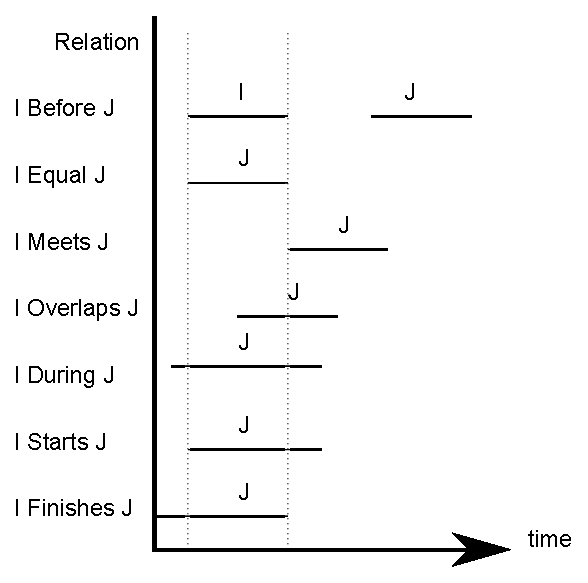
\includegraphics[width=0.9\columnwidth]{graphs/allen.eps}
   \caption{The Allen relationships between two crisp intervals $I$ and $J$.  }
   \label{fig:allen-relationships}
 \end{figure}

To be able to query IS containing data representing time indications subject to uncertainty, a framework is necessary, able to represent uncertainties in time indications in a semantically sound way, without (much) information loss and able to temporally reason with such time indications in a semantically sound and usefull way~\cite{Dubois1983},~\cite{Dubois2003}. Although more proposals for such frameworks exist, the work presented in this paper focusses on just two: the \emph{ill-known constraint \emph{(IKC)} framework}~\cite{Pons2011} and the \emph{triangular model \emph{(TM)} framework}~\cite{DeTre2012}.

The work presented in this paper consists of a comparison of both frameworks, about the approaches they use to represent time intervals subject to uncertainty and to reason about the temporal relationships between such intervals and time intervals without uncertainty.

The structure of this paper is as follows: section \ref{sec:general-preliminaries} presents some general preliminaries and naming and notation conventions used in this paper. Sections \ref{sec:ikc} and \ref{sec:tm} introduce the IKC and TM frameworks respectively: both sections first introduce some specific preliminary concepts and techniques, then explain how the representation of time intervals by the framework is done and finally show how the evaluation of Allen relationships between an interval subject to uncertainty and one without uncertainty is done. In section \ref{sec:proposal}, both frameworks are compared: first their approaches to representing time intervals are compared, next their approaches to evaluating Allen relationships. Finally, section \ref{sec:conclusions} presents the principal conclusions of the presented work and some possible future work. 

%TODO: more references in the above part?
%TODO: include some form of proof or previous work with these statements?!

%The concept of the time has been widely studied \cite{Benthem1982}, \cite{Shackle1961}, \cite{Klein1994}. Moreover, humans beings manage temporal indications in an imprecise way \cite{Devos1998}. But when dealing with time in an Information System, some simplifications must to be done. The first thing to do is the discretization of the time line into time points or time intervals. Both approaches have been proved to be equivalent, although due to the nature of the smallest unit of time in a computer, a \emph{chronon}, the discretization of a time point returns a time interval.

%All the possible positions between two time intervals were studied by Allen \cite{Allen1983}, \cite{Allen1985}. As result, the thirteen Allen's Relations were obtained (See Table \ref{tab:allen-relations}) which are illustrated in Figure \ref{fig:allen-relationships}. In order to achieve a more intelligent processing of time, some theoretical frameworks are used to reason with time. First the possibility theory was employed in the reasoning with temporal information \cite{Dubois2003a}. Then, several proposals \cite{Schockaert2008}, \cite{nagypal2003}, \cite{Ohlbach2004}, \cite{Pons2011} studied how to extend the thirteen Allen's relations to the possibilistic case. Also rough set theory \cite{Pawlak1995} has been used to represent and reason about imperfect time intervals \cite{Qiang2009}, \cite{Qiang2010}.

%Although there exists several proposals to represent and visualize imperfect time intervals, in this paper we will focus on two: the ill-known constraint framework \cite{Pons2011} and the triangular model \cite{DeTre2012}. The first one is a theoretical framework that deals with temporal reasoning and the second one is a visual framework that represent imperfect time intervals in a two dimensional space. Both frameworks can be used to represent imperfect time intervals as well as temporal reasoning.

%The structure of this paper is the following. Section  \ref{sec:preliminaries} introduces the Ill-known constraint framework. Section \ref{sec:triangular-model} introduces the triangular model. Section \ref{sec:proposal} analyze both frameworks and shows the correspondences and differences between both frameworks. The section concludes with an example showing that the calculations made in both frameworks are equivalent. Finally, Section \ref{sec:conclusions} presents the main conclusions and the future work. 


%\begin{table}[h]
%\centering
%\begin{tabular}{|c|l|}
%\hline
%Name & Implementation \\ \hline 
%$I$ equals $J$ & if $s_i = s_j \wedge e_i = e_j $ \\
%$I$ starts $J$ & if $s_i = s_j \wedge e_i < e_j $ \\
%$I$ started by $J$ & if $s_i = s_j \wedge e_i > e_j $ \\
%$I$ finishes $J$ & if $s_i > s_j \wedge e_i = e_j $ \\
%$I$ finished by $J$ & if $s_i < s_j \wedge e_i = e_j $ \\
%$I$ meets $J$ & if $e_i = s_j $ \\
%$I$ met by $J$ & if $s_i = e_j $ \\
%$I$ overlaps $J$ & if $s_i < s_j \wedge e_i < e_j \wedge e_i > s_j $ \\
%$I$ overlapped by $J$ & if $s_i > s_j \wedge e_j < e_i \wedge s_i < e_j  $ \\
%$I$ during $J$ & if $s_i > s_j \wedge e_i < e_j $ \\
%$I$ contains $J$ & if $  s_i < s_j \wedge e_i > e_j$ \\
%$I$ before $J$ & if $e_i < s_j $ \\
%$I$ after $J$ & if $s_i > e_j $ \\
%\hline
%\end{tabular}
%\caption{Allen's relations represented in the framework. $I = \left[s_i, e_i\right]$, $J=  \left[s_j, e_j\right]$}
%\label{tab:allen-relations}
%\end{table}

